\AtBeginSubsection[] { %
\begin{frame}[t,noframenumbering]
\Title{Plan}
\Block{4cm,2cm}{8cm}{
    \tableofcontents[
        currentsection,
        currentsubsection,
        % hideothersubsections,
        sectionstyle=show/shaded,
        subsectionstyle=show/shaded/hide
    ]
}
\end{frame}
}
% \AtBeginSubsection[] { %
%   \begin{frame}[noframenumbering]
%     \frametitle{Plan}
%     \tableofcontents[
%     currentsection,
%     currentsubsection,
%     % hideothersubsections,
%     sectionstyle=show/shaded,
%     subsectionstyle=show/shaded/hide]
%   \end{frame}}
 
\subsection{Attack Methods}

% \begin{frame}
%     \begin{center}
%         \Large Attacks on Masked \\
%         White-box Implementations
%     \end{center}
% \end{frame}

% \begin{frame}{Attacks I}
% {\bf Combinatorial attacks:}

% \begin{itemize}
%     \item (partially) guess locations of the shares
%     \item {\bf probabilistic}: correlation with predictable values
%     \item {\bf exact}: time-memory trade-off
% \end{itemize}

% \vspace{0.5cm}

% \pause

% {\bf Fault attacks:}

% \begin{itemize}
%     \item {\bf new application:} \alert{recover locations} of the shares
%     \item 1- and 2- share fault injections
%     \item applicability depends on protections
% \end{itemize}

% \end{frame}


\begin{frame}[t]
\Title{(Generalized) Differential Computation Analysis (DCA)}

\Center{
\only<1>{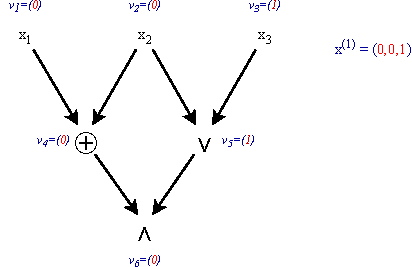
\includegraphics[height=7cm,page=1]{figures/CircuitDCA-crop.pdf}}
\only<2>{\includegraphics[height=7cm,page=2]{figures/CircuitDCA-crop.pdf}}
\only<3>{\includegraphics[height=7cm,page=3]{figures/CircuitDCA-crop.pdf}}
}
\end{frame}



\begin{frame}
\Title{The Linear Algebra Attack}
\only<4>{\Footnote{
Goubin et al: How to Reveal the Secrets of an Obscure White-Box Implementation. \href{https://eprint.iacr.org/2018/098.pdf}{(ePrint 2018/098)}
}}
\CenterBlock{12cm}{
\vspace{0.5cm}
\begin{itemize}
    \item consider Boolean masking ({\bf linear} decoder)
    \item matching with a \textcolor{green!35!black}{predictable value} $\color{green!35!black}{s}$:
        \\a basic linear algebra problem:
        $$\color{blue}{M}\times \color{red}{z} = \color{green!35!black}{s}, ~~~~\color{blue}{M = [v_1 ~\mid~ \ldots ~\mid~ v_n]}$$
    \pause
    \item $\color{blue}{v_i}$ is the vector of values computed in a node $i$ of the circuit
    \item $\color{red}{z}$ is the vector indicating \textcolor{red}{locations} of shares among nodes of the circuit
\end{itemize}
}
\pause
\center{\alert{higher number of shares does not prevent the attack...}}

\end{frame}


% \begin{frame}
% \begin{center}
% \Large Generalizations of the Linear Algebra Attack \\
% \end{center}

% \begin{itemize}
%     \item {\bf nonlinear decoders}, through linearization technique
%     \item {\bf approximately linear decoders}, through LPN algorithms
%     \pause
%     \item {\bf semi-linear decoders:}
%     \begin{enumerate}
%         \item assume $s\cdot r$ is computed/shared in the circuit, where
%         \item $s$ is a {\color{PineGreen}predictable} value
%         \item $r$ is \alert{unpredictable} (pseudorandom, $\approx$ uniform)
%         \pause
%         \item choose plaintexts $p_1,\ldots,p_D$ such that: \\
%             $s(p_i) = 0$ ~~ for $1 \le i \le D-1,$ \\
%             $s(p_i) = 1$ ~~ for $i = D$.
%         \item $s \cdot r$ will be equal to $(0,0,\ldots,0,1)$ with $\Pr=1/2$
%         \item if $s$ is guessed wrong, such vector is unlikely to be a solution
%     \end{enumerate}
% \end{itemize}

% \end{frame}
